\begin{figure}[h,centering]
  \caption{The Correspondence Theorem}
  \label{fig:correspthm}
  \begin{center}
    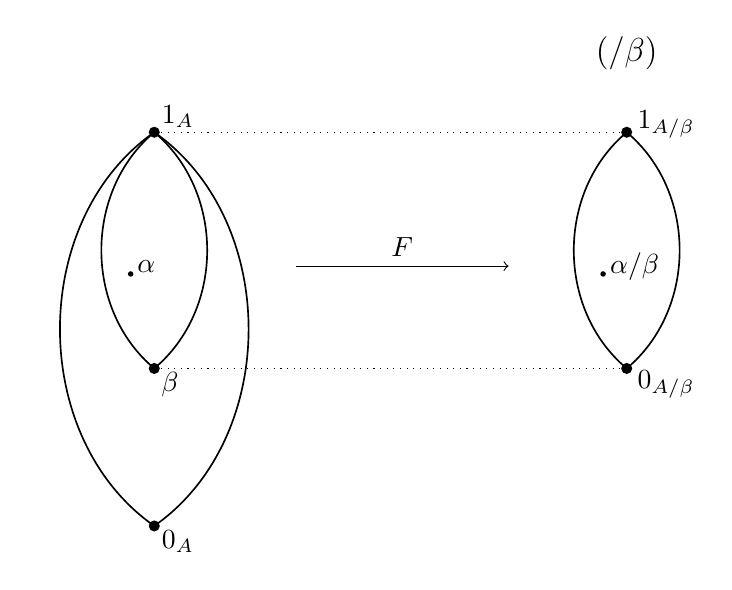
\begin{tikzpicture}
      \draw[font=\large] (0,6) node {$\Con \bA$};
      \draw[font=\large] (6,6) node {$\Con (\bA/\beta)$};
      \draw[semithick] (0,5) to [out=215,in=145] (0,0); \fill (0,0) circle (2pt);
      \draw[semithick] (0,0) to [out=35,in=-35] (0,5); \fill (0,5) circle (2pt);
      \draw[semithick] (0,5) to [out=220,in=140] (0,2); 
      \draw[semithick] (0,2) to [out=40,in=-40] (0,5); 
      \fill (-.3,3.2) circle (1pt); \draw (-.1,3.3) node {$\alpha$};
      \fill (0,2) circle (2pt); \draw (0.2,1.8) node {$\beta$};
      \draw (0.3,-.2) node {$0_A$}; \draw (0.3,5.2) node {$1_A$};

      \fill (5.7,3.2) circle (1pt); 
      \draw (6.1,3.3) node {$\alpha/\beta$};
      \draw (6.5,1.8) node {$0_{A/\beta}$}; \draw (6.5,5.1) node {$1_{A/\beta}$};
      \draw[semithick] (6,5) to [out=220,in=140] (6,2); \fill (6,2) circle (2pt);
      \draw[semithick] (6,2) to [out=40,in=-40] (6,5); \fill (6,5) circle (2pt);

      \draw[dotted] (0,5) -- (6,5);
      \draw[dotted] (0,2) -- (6,2);
      % \path[->,font=\scriptsize] (1.8,3.3) edge node[above] {$F$} (4.5,3.3);
      \path[->] (1.8,3.3) edge node[above] {$F$} (4.5,3.3);
    \end{tikzpicture}
  \end{center}
\end{figure}
